\subsection{Модуль обнаружения ошибок при обработке документа} \label{research_feedback}

При обработке документов автоматиизирвоанным способом существует возможность обнаружения ошибок на стадии редактирования, т.е. до отправки документа далее по цепочке обработки. В таком случае ошибка либо устраняется автоматически, либо создаётся новая задача на устранение ошибки тому же редактору, который эту ошибку допустил.

\vspace{\baselineskip}
Одной из разновидностей ошибки такого рода является некорректное обращение к полям документа. Стоит отметить, что речь здесь идёт не о метаданных, сопровождающих документ, а об информации, содержащейся непосредственно в документе.Например, для совместной работы, описанной в гл. \ref{research_competition}, таким обращением будет считаться попытка редактирвоания полей документа, обработкой которых уже занимается другой редактор.

\vspace{\baselineskip}
Для эксперимента были рассмотрены две схемы: одна -- <<классическая>>, без обнаружения ошибок такого рода (многие СЭД не предоставляют подобного сервиса, регулируя только поля метаданных, см. табл. \ref{table:products}), другая -- согласно описанной выше схеме, реализованная в описываемой разработке.

\vspace{\baselineskip}
На рис. \ref{img:feedback_old_scheme} представлена схема без автоматизированного обнаружения ошибок. Возврат на доработку при такой организации возможен, но осуществляется в ручном режиме: редактор, получивший на вход задания документ с ошибкой, отправляет его на переработку предыдущему редактору (в реальной системе он будет передавать документ соседнему звену в обратном направлении, однако как показывает практика, в случае подчинения низших звеньев высшим документ будет возвращаться до первого редактора). Последний редактор в случае допуска ошибки получит неверный документ, на схеме приёмник таких результатов обозначен $sink$. Корректно обработанные заявки приходит в пункт $sink2$. Разветвления после обработчиков работают по вероятностному принципу с вероятностью обнаружения ошибки $P_{txt}'$.
 
\begin{figure}[h!]
  \centering
  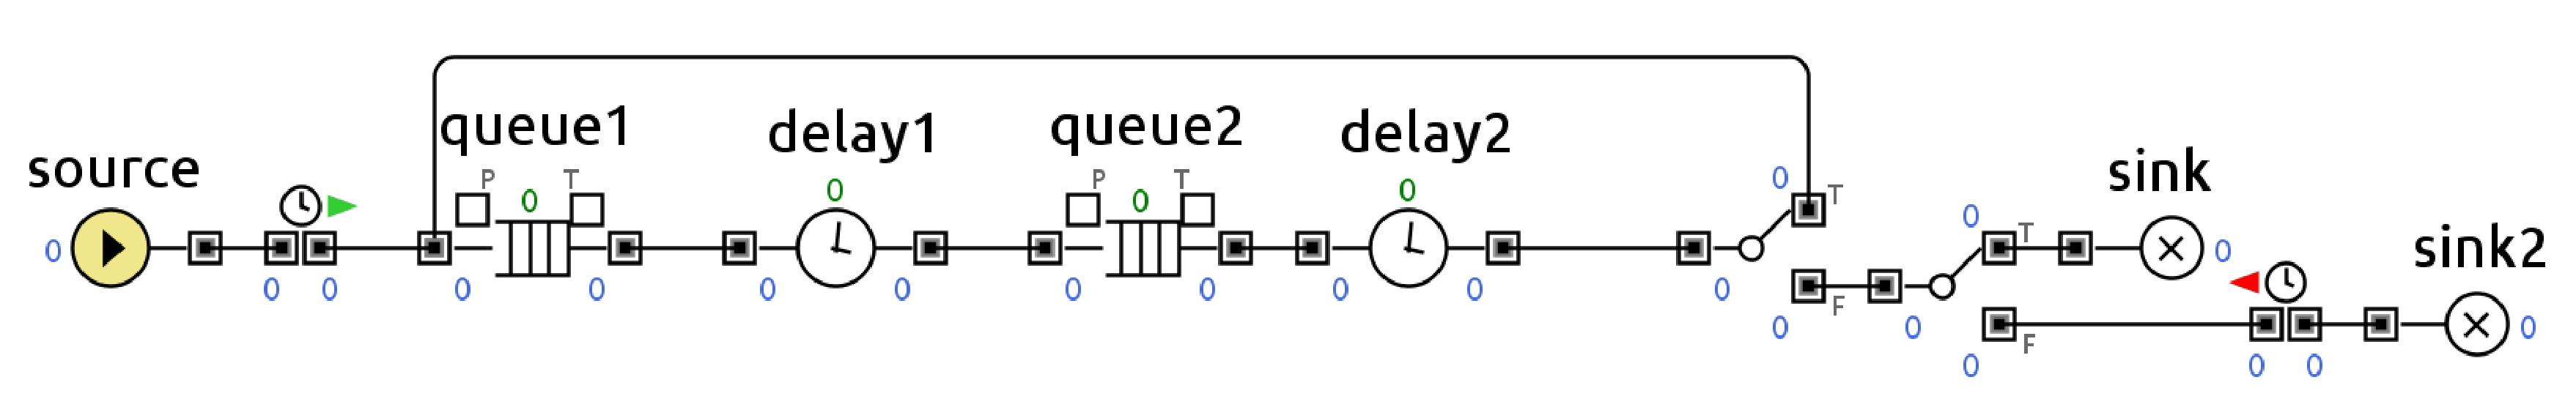
\includegraphics[width=1\textwidth]{feedback_old_scheme}
  \caption{Схема коррекции ошибок ручным методом}
  \label{img:feedback_old_scheme}
\end{figure}

\vspace{\baselineskip}
В случае автомтизированного обнаружения ошибок (рис. \ref{img:feedback_new_scheme}) задание на переработку генерируется автоматически для того редактора, который допустил ошибку. Таким образом, даже последний редактор в цепочке имеет возможность исправить допущенную ошибку перед публикацией документа.

\begin{figure}[h!]
  \centering
  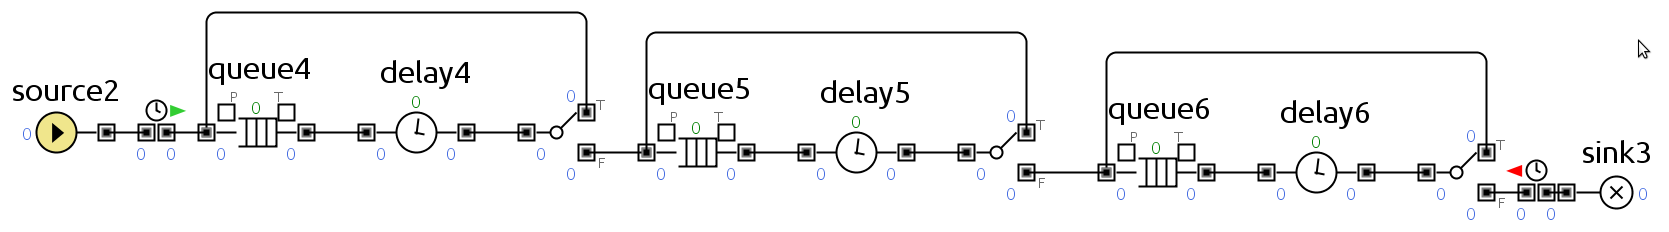
\includegraphics[width=1\textwidth]{feedback_new_scheme}
  \caption{Схема коррекции ошибок автоматизированным методом}
  \label{img:feedback_new_scheme}
\end{figure}

\vspace{\baselineskip}
Одним из показателей эффективности метода организации процесса обработки документов является число корректно обработанных заявок. Как и в случае совместной работы пользователей, заявки генерируются по одной за полчаса реального времени, моделируется один рабочий день (с 9:00 до 18:00). Параметры обработчиков совпадают с описанными в гл. \ref{research_competition}. Результат моделирования представлен на рис. \ref{img:feedback_done}.

\begin{figure}[h!]
  \centering
  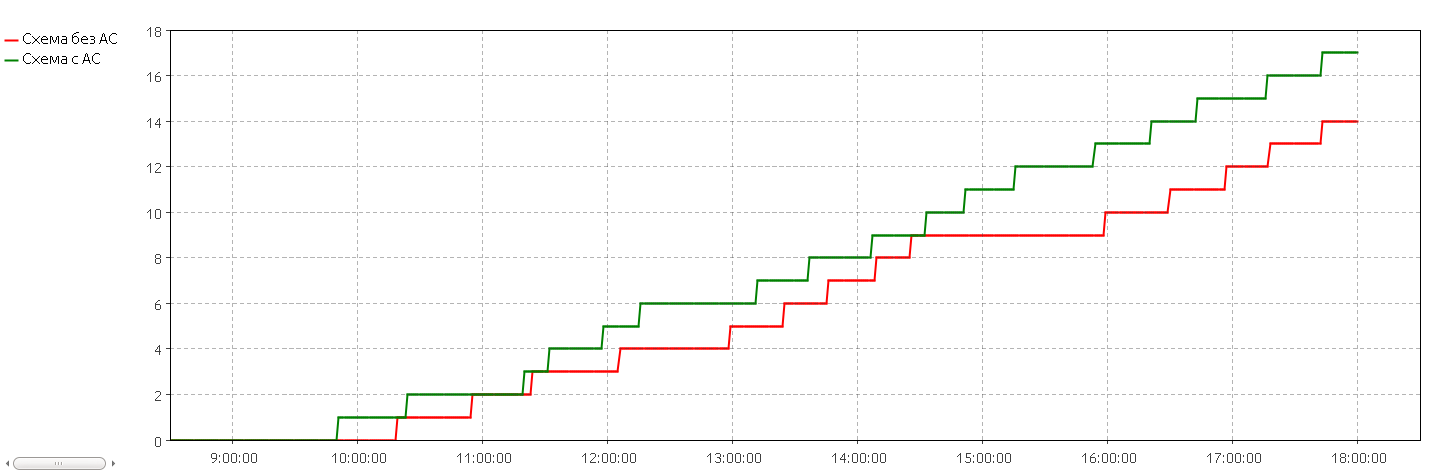
\includegraphics[width=1\textwidth]{feedback_done}
  \caption{Число обработанных заявок в схемах с обратной связью}
  \label{img:feedback_done}
\end{figure}

\vspace{\baselineskip}
Как видно из рисунка, схема с автоматизирвоанным обнаружением ошибок позволяет обработать больше заявок за ограниченный промежуток времени. Также можно заметить, что частота, с которой заявкам присваивался статус <<корректно обработанная>>, выше в схеме с АС. Это позволяет предположить, что среднее время обработки одной заявки при такой организации меньше, чем при ручном обнаружении ошибок. Данная гипотеза подтверждается графиком, приведённым на рис. \ref{img:feedback_mean}.

\begin{figure}[h!]
  \centering
  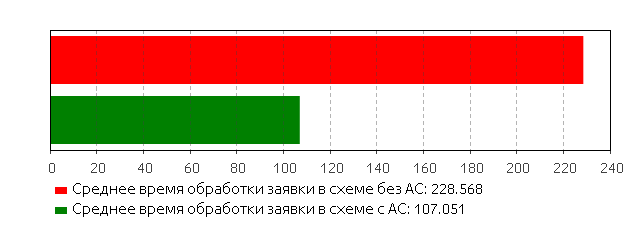
\includegraphics[width=1\textwidth]{feedback_mean}
  \caption{Среднее время обработки одной заявки в схемах с обратной связью}
  \label{img:feedback_mean}
\end{figure}

\vspace{\baselineskip}
Уменьшение времени обработки заявки происходит за счёт того, что в случае необходимости исправления ошибки над документом работает один редактор из цепочки (тот, который допустил ошибку), а не все. Более того, среднее время обработки заявки в схеме без АС можно считать заниженным, т.к. в нём не учтено время поиска ошибки, а сама вероятность её обнаружения оценена довольно высоко -- наравне с АС. 

\vspace{\baselineskip}
Таким образом, для снижения времени обработки заявок целесообразно использовать систему автоматического обнаружения ошибок.